\chapter{The Lucene Search Library}\label{chap:lucene}

\firstchar{A}pache Lucene is a search library written in Java.  Due to
its performance, configurability and generous licensing terms, it has
become very popular in both academic and commercial settings.  In this
section, we'll provide an overview of Lucene's components and how to
use them, based on a single simple hello-world type example.  

Lucene provides search over documents.  A document is essentially a
collection of fields, where a field supplies a field name and value.
Lucene manages a dynamic document index, which supports adding
documents to the index and retrieving documents from the index using a
highly expressive search API.  

Lucene does not in any way constrain document structures.  An index
may store a heterogeneous set of documents, with any number of
different fields which may vary by document in arbitrary ways. 
Lucene can store numerical and binary data as well as text, 
but in this tutorial we will concentrate on text values.

What actually gets indexed is a set of terms.  A term combines a field
name with a token that may be used for search.  For instance, a title
field like \stringmention{Molecular Biology, 2nd Edition} might yield
the tokens \stringmention{molecul}, \stringmention{biolog},
\stringmention{2}, and \stringmention{edition} after case
normalization, stemming and stoplisting.  The index structure provides
the reverse mapping from terms, consisting of field names and tokens,
back to documents.  To search this index, we construct a term composed
of the field title and the tokens resulting from applying the same
stemming and stoplisting to the text we are looking for.

\section{Fields}

A document is a collection of fields.
Search and indexing is carried out over these fields.
All fields in Lucene are instances of the \code{Fieldable} interface
in the package \code{org.apache.lucene.document}.  This interface is 
implemented by the abstract class \code{AbstractField} and the
two final classes \code{Field} and \code{NumericField} which inherit
from it.  In this tutorial we cover the use of the class \code{Field}
to index and store text.

For example, a MEDLINE citation might be stored as a series
of fields: one for the name of the article, another for name of
the journal in which it was published, another field for the authors
of the article, a pub-date field for the date of publication, a field
for the text of the article's abstract, and another field for the list
of topic keywords drawn from Medical Subject Headings (MeSH).  Each of
these fields would get a different name, and at search time, the
client could specify that it was searching for authors or titles or
both, potentially restricting to a date range and set of journals
by constructing search terms for the appropriate fields and values.

\subsection{Constructing Fields}

A field requires all of its components to be specified in the
constructor.  Even so, fields are defined to be mutable so that their
values, but not their field names, may be reset after construction.

The field constructor takes the field name, value, and a set of flags
which specify how it will be saved in the index.
These indexing flags are discussed in a subsequent section.

There are also several utility constructors that provide default
values for the flags in addition to those taking the text value as a
\code{Reader}.  There is also a public constructor that takes a
\code{TokenStream} (see \refsec{lucene-analysis}) rather than a
string.%
%
\footnote{According to the javadoc,
this is useful for pre-analyzed fields.
Users must be careful to make sure the token stream provided is
consistent with whatever analysis will happen at query time.}
%
An additional constructor takes a boolean flag controlling whether
the field's name is interned or not (see \refsec{string-intern}), with
the default setting being \code{true}.


\subsection{Field Names and Values}

Each constructor for a field requires a name for the field.  At search
time, the supplied field name restricts the search to particular
fields.  

Each constructor for a field requires a value for the field
which may be supplied as a Java \code{String} or \code{Reader}.%
%
\footnote{We recommend not using a \code{Reader}, because the policy
  on closing such readers is confusing.  It's up to the client to
  close, but the close can only be done after the document has been
  added to an index.  Making fields stateful in this way introduces a
  lifecycle management problem that's easily avoided.  Very rarely
  will documents be such that a file or network-based reader may be
  used as is in a field; usually such streams are parsed into fields
  before indexing, eliminating any performance advantage readers might
  have.}
%
The value for a binary field is supplied as a byte array slice.

\subsection{Indexing Flags}

As of version 3.0 of Lucene, the constructor for a field has three
arguments that control how a term is indexed and/or stored.  These
arguments are specified using nested enum instances in the
\code{Field} class.

\subsubsection{The \code{Field.Store} Enum}

All fields are marked as to whether their raw value is stored in the
index or not.  Storing raw values allows you to retrieve them at
search time, but may consume substantial space.  

The enum \code{Field.Store} is used to mark whether or not to store
the value of a field.  Its two instances, \code{Store.YES} and
\code{Store.NO}, have the obvious interpretations.

\subsubsection{The \code{Field.Index} Enum}

All fields are also marked as to whether they are indexed or not.  A
field must be indexed in order for it to be searchable.  While it's
possible to have a field that is indexed but not stored, or stored but
not indexed, it's pointless to have a field that is neither stored nor
indexed.

Whether a field is indexed is controlled by an instance of the
\code{Field.Index} enum.  The value \code{Index.NO} turns off indexing
for a field.  The other values all turn on indexing for a field.
Where they vary is how the terms that are indexed are pulled out of
the field value.  The value \code{Index.ANALYZED} indexes a field with
tokenization turned on (see \refsec{lucene-analysis}).  The value
\code{Index.NOT\_ANALYZED} causes the field value to be treated like a
single token; it's primarily used for identifier fields that are not
decomposed into searchable terms.

\subsubsection{The \code{Field.TermVector} Enum}

The final specification on a field is whether to store term vectors or
not, and if they are stored, what specifically to store.  A term
vector stores a list of the document's terms and number of occurrences
in that document.  Term vectors can also store token position.  They
may be useful for downstream processing like results clustering, 
finding documents that are similar to a known document, or document
highlighting.

Whether to use term vectors is controlled by an instance of the enum
\code{Field.TermVector}.  The default is not to store term vectors,
corresponding to value \code{TermVector.NO}.  Because we do not need
term vectors for our simple demo, we use a
constructor for \code{Field} which implicitly sets the term vector
flag to \code{TermVector.NO}.

\subsection{Field Getters}

Once we have a field, we can access the components of it such as its
name, value, whether its indexed, stored, or tokenized, and whether
term vectors are stored.  These methods are all specified in the
\code{Fieldable} interface.  For instance, \code{name()} returns
a field's name, and \code{stringValue()} its value.%
%
\footnote{For fields constructed with a \code{Reader} for a value, the
  method \code{stringValue()} returns \code{null}.  Instead, the
  method \code{readerValue()} must be used.  Similarly, the methods
  \code{tokenStreamValue()} and \code{binaryValue()} are used to
  retrieve values of fields constructed with token streams or byte
  array values.  The problem with classes like this that that allow
  disjoint setters (or constructors) is that it complicates usage for
  clients, who now have to check where they can get their data.
  Another example of this anti-pattern is Java's built-in XML
  \code{InputSource} in package \code{org.xml.sax}.}
%

There are convenience getters derived from the flag settings.  For
instance, \code{isIndexed()} indicates if the field is indexed, and
\code{isTokenized()} indicates whether the indexing involved analysis
of some sort.  The method \code{isStored()} indicates if the value is
stored in the index, and \code{isTermVectorStored()} whether the term
vector is stored in the index.

\section{Documents}

In Lucene, documents are represented as instances of the final class
\code{Document}, in package \code{org.apache.lucene.document}.

\subsection{Constructing and Populating Documents} 

Documents are constructed using a zero-arg constructor
\code{Document()}.  Once a document is constructed, the method
\code{add(Fieldable)} is used to add fields to the document.

Lucene does not in any way constrain document structures.  An index
may store a heterogeneous set of documents, with any number of
different fields which may vary by document in arbitrary ways.  It is
up to the user to enforce consistency at the document collection
level.  

A document may have more than one field with the same name added to
it.  All of the fields with a given name will be searchable under that
name (if the field is indexed, of course).  The behavior is
conceptually similar to what you'd get from concatenating all the
field values; the main difference is that phrase searches
don't work across the concatenated items.

\subsection{Accessing Fields in Documents}

The \code{Document} class provides a means of getting fields by name.
The method \code{getFieldable(String)} returns the field for a
specified name.  If there's no field with the specified name, it
returns \code{null} rather than raising an exception.

The return type is \code{Fieldable}, but this interface provides
nearly the same list of methods as \code{Field} itself, so there is
rarely a need to cast a fieldable to a field.  

If there is more than one field in a document with the same name, the
simple method \code{getFieldable(String)} only returns the first one
added.  The method \code{getFieldables(String)} returns an array of
all fields in a document with the given name.  It's costly to
construct arrays at run time (in both space and time for allocation
and garbage collection), so if there is only a single value, the
simpler method is preferable.


\subsection{Document Demo}

We provide a simple demo class, \code{DocDemo}, which illustrates
the construction, setting and accessing of fields and documents.

\subsubsection{Code Walkthrough}

The \code{main()} method starts by constructing a document and
populating it.
%
\codeblock{DocDemo.1}
%
After constructing the document, we add a sequence of fields,
including a title field, two author fields, a field for the name of
the journal, several fields storing mesh terms, and a field storing
the document's PubMed identifier.
These terms are all stored
and analyzed other than the identifier, which is not analyzed.

After constructing the document, we loop over the fields and
inspect them.
%
\codeblock{DocDemo.2}
%
Note that the access is through the \code{Fieldable} interface.
We include the calls to the relevant methods, 
but omit the actual print statements.

\subsubsection{Running the Demo}

The Ant target \code{doc-demo} runs the demo.  
%
\commandlinefollow{ant doc-demo}
\begin{verbatim}
name=title value=Fast and Accurate Read Alignment
     indexed=true store=true tok=true termVecs=false
name=author value=Heng Li
     indexed=true store=true tok=true termVecs=false
...
name=mesh value=genomics/methods
     indexed=true store=true tok=true termVecs=false
name=mesh value=sequence alignment/methods
     indexed=true store=true tok=true termVecs=false
name=pmid value=20080505
     indexed=true store=true tok=false termVecs=false
\end{verbatim}
%
We've elided three fields, marked by ellipses.



\section{Analysis and Token Streams}\label{section:lucene-analysis}

Lucene employs analyzers to convert the text value
of a fields marked as analyzed to a stream of tokens.  At indexing
time, Lucene is supplied with an implementation of the abstract base
class \code{Analyzer} in package \code{org.apache.lucene.analysis}.
An analyzer maps a field name and text value to a \code{TokenStream},
also in the \code{analysis} package, from which the terms to be
indexed are retrieved using an iterator-like pattern.

\subsection{Token Streams and Attributes}

Before version 3.0 of Lucene, token streams had a string-position
oriented tokenization API, much like LingPipe's tokenizers.  Version
3.0 generalized the interface for token streams and other basic
objects using a very general design pattern based on attributes of
other objects.
%
\footnote{The benefit of this pattern is not in its use, which is less
  convenient than a direct implementation.  The advantage of Lucene's
  attribute pattern is that it leaves enormous flexibility for the
  developers to add new features without breaking backward
  compatibility.}

\subsubsection{Code Walkthrough}

To see how the tokenization process works,
we provide a sample class \code{LuceneAnalysis} that applies an
analyzer to a field name and text input and prints out the resulting
tokens.  The work is done in a simple \code{main()} with two
arguments, the field name, set as the string variable
\code{fieldName}, and the text to be analyzed, set as the string
variable \code{text}.

The first step is to create the analyzer.
%
\codeblock{LuceneAnalysis.1}
%
Here we've used Lucene's \code{StandardAnalyzer}, in package
\code{org.apache.lucene.analysis.standard}, which applies case
normalization and English stoplisting to the simple tokenizer, which
pays attention to issues like periods and e-mail addresses.%
%
\footnote{See the tokenization chapter in the companion volume, {\it
    Natural Language Processing in LingPipe} for an overview of
  natural language tokenization in LingPipe, as well as adapters
  between Lucene analyzers and LingPipe tokenizer factories).}
%
Note that it's constructed with a constant for the Lucene version, as
the behavior has changed over time.

The standard analyzer, like almost all of Lucene's built-in analyzers,
ignores the name of the field that is passed in.  Such analyzers
essentially implement simple token stream factories, like LingPipe's
tokenizer factories.%
%
\footnote{It is unfortunate that Lucene does not present a token
  stream factory interface to produce token streams from text inputs.
  Then it would be natural to construct an analyzer by associating
  token stream factories with field names.  We follow this pattern in
  adapting LingPipe's tokenizer factories to analyzers in the companion
  volume, {\it Natural Language Processing with LingPipe}, in the
  section on adapting Lucene analyzers.

Lucene's sister package, Solr, which embeds Lucene in a client-server
architecture, includes a token stream factory interface
\code{TokenizerFactory}, which is very much like LingPipe's other than
operating over readers rather than character sequences and providing
Solr-specific initialization and configuration management.}


The next step of the \code{main()} method constructs the token stream
given the string values of the command-line arguments \code{fieldName}
and \code{text}.  
%
\codeblock{LuceneAnalysis.2}
%
We first have to create a \code{Reader}, which we do by wrapping the
input text string in a \code{StringReader} (from \code{java.io}).%
%
\footnote{Unlike the case for documents, there is no alternative to
  using readers for analysis.  It is common to use string readers
  because they do not maintain handles on resources other than their
  string reference.}
%
Then we use the analyzer to create a token stream from the field name
and text reader.  The next three statements attach attributes to the
token stream, specifically a term attribute,%
%
\footnote{As of version 3.1, the \code{TermAttribute} class was
  renamed \code{CharTermAttribute} because it holds objects of type
 \code{CharSequence}, which can be printed by the \code{toString}
  method.}
%
offset attribute and
position increment attribute.  These are used to retrieve the text of
a term, the span of the term in the original text, and the ordinal
position of the term in the sequence of terms in the document.  The
position is given by an increment from the previous position, and
Lucene uses these values for phrase-based search \ie{searching for a
fixed sequence of tokens in the given order without intervening
material}.

The last block of code in the \code{main()} method iterates through
the token stream, printing the attributes of each token it finds.
%
\codeblock{LuceneAnalysis.3}
%
The while loop continually calls \code{incrementToken()} on the token
stream, which advances to the next token, returning \code{true} if
there are more tokens.  The body of the loop just pulls out the
increment, start and end positions, and term for the token.  The rest
of the code, which isn't shown, just prints these values.  this
pattern of increment-then-get is particularly popular for tokenizers;
LingPipe's tokenizers use a similar model.  

\subsubsection{Running the Demo}

It may be run from the Ant target \code{lucene-analysis}, with
the arguments provided by properties \code{field.name} and 
\code{text} respectively.

\commandlinefollow{ant -Dfield.name=foo -Dtext="Mr.\ Sutton-Smith will pay \$1.20 for the book." lucene-analysis}
\begin{verbatim}
Mr. Sutton-Smith will pay $1.20 for the book.
012345678901234567890123456789012345678901234
0         1         2         3         4

 INCR (START,   END) TERM         INCR (START,   END) TERM
    1 (    0,     2) mr              2 (   22,    25) pay
    1 (    4,    10) sutton          1 (   27,    31) 1.20
    1 (   11,    16) smith           3 (   40,    44) book
\end{verbatim}
%
The terms are all lowercased, and non-word-internal punctuation has
been removed.  The stop words \charmention{will}, \charmention{for}
and \charmention{the} are also removed from the output.  Unlike
punctuation, when a stop word is removed, it causes the increment
between terms to be larger.  For instance, the increment between
\charmention{smith} and \charmention{pay} is 2, because the stopword
\charmention{will} was removed between them.  The start (inclusive)
and end (exclusive) positions of the extracted terms is also shown.


\section{Directories}\label{section:lucene-directory}

Lucene provides a storage abstraction on top of Java in the abstract
base class \code{Directory} in the \code{org.apache.lucene.store}
package.  Directories provide an interface that's similar to an
operating system's file system.

\subsection{Types of Directory}

The \code{FSDirectory} abstract base class, also in package
\code{store}, extends \code{Directory} to support implementations
based on a file system.  This is the most common way to create a
directory in Lucene.  The implementation \code{RAMDirectory}, also in
\code{store} supports in-memory directories, which are efficient, but
less scalable than file-system directories.  The package
\code{org.apache.lucene.store} contains several specialized
implementations.

\subsection{Constructing File-System Directories}

An instance of a file-system directory may be created using the
factory method \code{FSDirectory.open(File)}, which returns an
implementation of \code{FSDirectory}.
As of Lucene 3.6, this method returns a specific 
\code{FSDirectory} implementation,
based on your environment and the
known limitations of each implementation.

At construction, all \code{FSDirectory} implementations are 
supplied with a File and a \code{LockFactory} object which
specifies how the files on the file system will be locked.
The \code{LockFactory} class is an abstract class.
Several implementations are provided in the package
\code{org.apache.lucene.store}.
Convenience constructors supply a default \code{LockFactory}.
As of Lucene 3.6, this is a
\code{NativeFSLockFactory}.


\section{Indexing}

Lucene uses the \code{IndexWriter} class in
\code{org.apache.lucene.index} to add documents to an index and
optimize existing indexes.  Documents do not all need to be added at
once --- documents may be added to or removed from an existing index.
We consider deleting documents in \refsec{lucene-delete}.

\subsection{Constructing an IndexWriter}

An IndexWriter is constructed from a \code{lucene.store.Directory} and
a \code{IndexWriterConfig} object which specifies the Lucene version
of the index, the default Analyzer, and how the IndexWriter uses
memory and processing resources during indexing.  The
\code{IndexWriterConfig} constructor takes the Lucene version and the
default analyzer as arguments and sets its properties to default
values accordingly.  Getter and setter methods are used to query and
update these properties.

\subsection{Merging and Optimizing}

Indexing maintains a small buffer of documents in memory,
occassionally writing the data in that batch of documents out to disk.
After enough such batches have been written to disk, Lucene
automatically merges the individual batches into bigger batches.
Then, after a number of larger chunks of index accumulate, these are
merged.  You can observe this behavior in your file browser if you're
using a disk directory for indexing a large batch of documents.  As
more documents are added, small index segments are continually added.
Then, at various points, these smaller indexes are merged into larger
indexes.

It's possible to control the size of the in-memory buffer and the
frequency of merges via setters on the \code{IndexWriterConfig}.

It's even possible to programatically merge two indexes from different
directories.  Lucene's \code{IndexWriter} class provides a handy
variable-argument-length method \code{addIndexes(IndexReader...)}
which adds indexes maintained by the specified readers to the index
writer.  Then, when the writer is optimized, the indexes will all
be merged into the writer's index directory.  

Being able to merge indexes makes it easy to split the indexing job
into multiple independent jobs and then either merge the results or
use all of the indexes together withour merging them (using a
\code{MultiReader}).


\subsection{Indexing Demo}

We provide a demo class \code{LuceneIndexing} that shows how basic
text indexing works.  

\subsubsection{Code Walkthrough}

The work is all done in the \code{main()} method, whIch starts by
constructing the index writer.
%
\codeblock{LuceneIndexing.1}
%
The two arguments correspond to the directory from which documents to
be indexed are read and the directory to which the Lucene index is
written.  We create a file-system-based directory using the index
directory (see \refsec{lucene-directory}).  

We then create a standard analyzer (see \refsec{lucene-analysis}).
In order to index all the text in a field, however long that field may be,
we need to wrap the standard analyzer in a \code{LimitTokenCountAnalyzer}
We set the maximum field length to \code{Integer.MAX\_VALUE}, the
largest possible value available.  

Next we specify the config for the index writer.  We call the
\code{setOpenMode} method with the enum constant
\code{IndexWriterConfig.OpenMode.CREATE} which causes the index writer
to create a new index or overwrite an existing one.  The other two
possible open modes enums are
\code{IndexWriterConfig.OpenMode.CREATE\_OR\_APPEND} which creates a
new index if one does not exist, else opens an existing index
and appends documents and \code{IndexWriterConfig.OpenMode.APPEND}
which opens an existing index.

For both the standard analyzer and the index writer
config we pass in a Lucene version constant.%
%
\footnote{The Lucene version constant supplied to components
in an application can differ by component.
For components used for both search and indexing it is critical
that the Lucene version is the same in the code that is called
at indexing time and the code that is called at search time.}
%
Finally, we create an index writer from the directory and the
index writer config.

Constructing the index may throw all three exceptions listed on the
\code{main()} method.  The first two exceptions are Lucene's, and both
extend \code{IOException}.  You may wish to catch them separately in
some cases, as they clearly indicate what went wrong. A
\code{CorruptIndexException} will be thrown if we attempt to open an
index that is not well formed.  A \code{LockObtainFailedException}
will be thrown if the index writer could not obtain a file lock on the
index directory.  A plain-old Java \code{IOException} will be thrown
if there is an underlying I/O error reading or writing from the files
in the directory.

The second half of the \code{main()} method loops over the files
in the specified document directory, converting them to documents
and adding them to the index.
%
\codeblock{LuceneIndexing.2}
%
We keep a count of the number of characters processed in the variable
\code{numChars}.  We then loop is over all the files in the specified
document directory.  For each file, we get its name and its text
(using LingPipe's static \code{readFromFile()} utility method, which
converts the bytes in the file to a string using the specified
character encoding, here ASCII).  

We then create a document and add the file name as an unanalyzed field
and the text as an analyzed field.  After creating the document, we
call the \code{addDocument(Document)} method of the index writer to
add it to the index.

After we've finished indexing all the files, we call the index
writer's \code{forceMerge(int)} method, followed by \code{commit}.
The argument to \code{forceMerge} is 1, so that the index will be merged down
into a single segment, 
resulting in a smaller index with better search performance.  
This is a costly operation.
The amount of free space required is two to three times the size of
the directory that the index writer is opened on.
When the merge completes, both the pre-merge and newly merged indexes exist.
Because Lucene allows search to proceed independently of indexing,
Lucene search components may have index readers open on the same directory.
These search components will be operating on the index that existed when they were opened
and will not see any changes made to the directory by the index writer
until the call to \code{commit}, which syncs all referenced index files.
At this point old indexes will be deleted, freeing up space.

We then close the index
writer using the \code{close()} method, which may throw an
\code{IOException}; the \code{IndexWriter} class is declared to
implement Java's \code{Closeable} interface, so we could've used
LingPipe's \code{Streams.closeSilently()} utility method to close it
and swallow any I/O exceptions raised.

Finally, we get the number of documents that are in the current index
using the method \code{numDocs()}; if documents were in the index when
it was opened, these are included in the count.  We also print out 
other counts, such as the number of characters, (print statements omitted
from above code listing).

\subsubsection{Running the Demo}

The Ant target \code{lucene-index} runs the indexing demo.  It
supplies the values of properties \code{doc.dir} and \code{index.dir}
to the program as the first two command-line arguments.  We created a
directory containing the 85 {\it Federalist Papers}, and use them
as an example document collection.
%
\commandlinefollow{ant -Ddoc.dir=../../data/federalist-papers/texts -Dindex.dir=temp.idx lucene-index}
\begin{verbatim}
Index Directory=/Users/mitzimorris/aliasi/lpbook/src/applucene/temp.idx
Doc Directory=/Users/mitzimorris/aliasi/lpbook/data/federalist-papers/texts
num docs=85
\end{verbatim}
%
Lucene's very fast.  On a workstation, it takes less than a second to
run the demo, including forking a new JVM.  On my wimpy notebook,
it takes two seconds. The run indexed 85
documents consisting of approximately 1.1 million words total.

After indexing, we can look at the contents of the index directory,
showing file size in kilobytes.
%
\commandlinefollow{export BLOCKSIZE=1024; ls -s temp.idx}
\begin{verbatim}
total 1544
1160 _0.fdt
   4 _0.fdx
   4 _0.fnm
  84 _0.frq
   4 _0.nrm
 192 _0.prx
   4 _0.tii
  84 _0.tis
   4 segments.gen
   4 segments_1
\end{verbatim}

%
These files contain binary representations of the index.  
The file segements.gen is a global file which contains the generation number of the index.
The file segments\_1 contains the per-commit list of segments.

The per-segment files begin with an underscore and have suffixes
which identify the type of data they contain.
The field info file, suffix \code{.fnm}, contains the field names and infos.
The term dictionary files, \code{.tis} and \code{.tii}, are used to navigate the index to
retrieve information for each term.
Term frequencies are stored in the \code{.frq} file
and term positions are stored in the \code{.prx} file.
Normalization factors used for scoring are stored in the \code{.nrm} file.
The files \code{.fdt} and \code{.fdx} contain the raw text data for the stored fields.
These last two are not used by Lucene for index search and scoring, they are only
for retrieval of search results.

The index takes up 1.5M total disk space.
Most of this space is used for the stored fields file, 1.2M in size,
which is slightly smaller than the raw text files themselves.
\commandlinefollow{du -sh ../../data/federalist-papers/texts}
\begin{verbatim}
1.3M	../../data/federalist-papers/texts
\end{verbatim}

\subsection{Luke}

Luke is an index browser for Lucene, also written in Java.
Downloads are available from \url{http://code.google.com/p/luke/}.
It provides a quick and easy way to explore the contents of the index.

\begin{figure}[!hb]
%\begin{center}
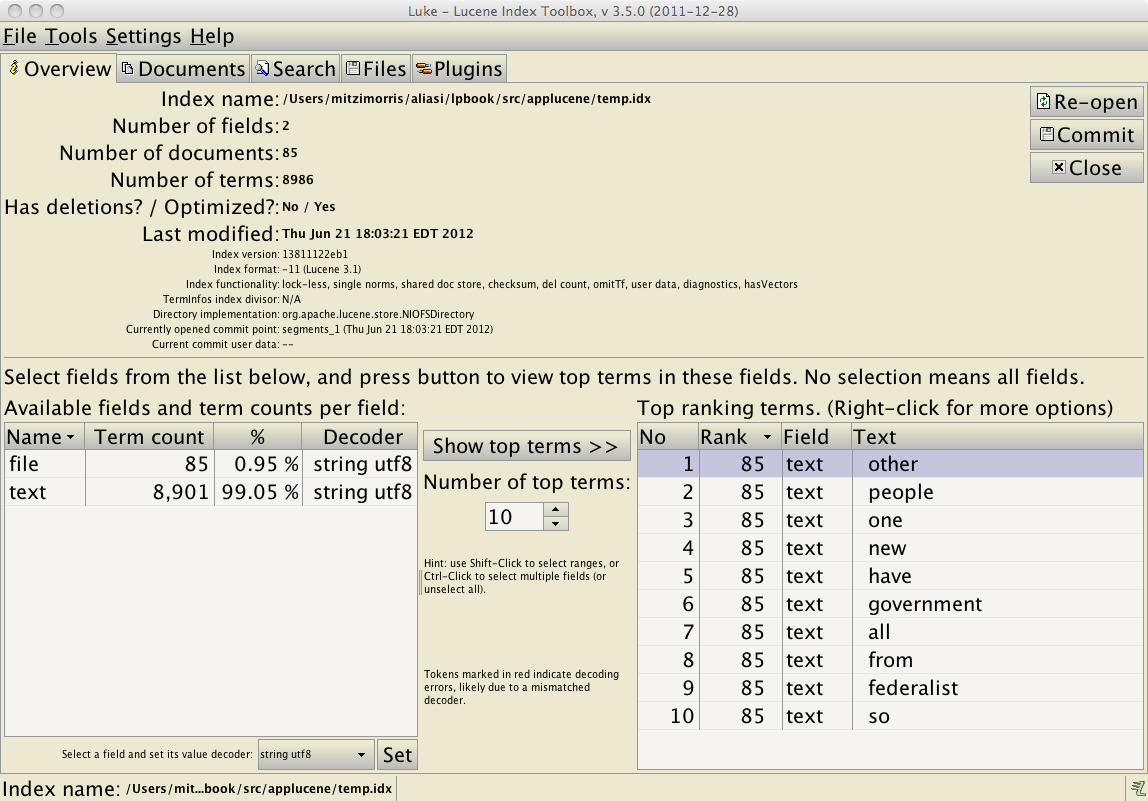
\includegraphics[width=5.0in]{pngs/luke1.png}
%\end{center}%
\vspace*{-18pt}
\caption{Screenshot of Luke index brower, showing overview of index temp.idx}
\end{figure}

\subsection{Duplicate Documents}

If we were to run the demo program again, each of the documents would
be added to the index a second time, and the number of documents
reported will be 170 (twice the initial 85).  Although a Lucene index
provides identifiers for documents that are unique (though not
necessarily stable over optimizations), nothing in the index enforces
uniqueness of document contents.  Lucene will happily create another
document with the same fields and values as another document.  It
keeps them separate internally using its own identifiers.

\section{Queries and Query Parsing}

Lucene provides a highly configurable hybrid form of search that
combines exact boolean searches with softer, more
relevance-ranking-oriented vector-space search methods.  
All searches are field-specific, because Lucene indexes terms and 
a term is comprised of a field name and a token.%
%
\footnote{Given that search is carried out over terms, 
 there's no way to easily have a query search over all fields.
 Instead, field-specific queries must be disjoined to achieve this
 effect.  Scoring for this approach may be problematic because
 hits on a shorter field  will have a higher score than hits on a longer field.
 Another approach is to denormalize the documents by creating
 synthetic fields that concatenate the value of other fields.}
%

\subsection{Constructing Queries Programatically}

Queries may be constructed programatically using the dozen or so
built-in implementations of the the \code{Query} abstract base class
from the package \code{org.apache.lucene.search}.  

The most basic query is over a single term in a single field.  This
form of query is implemented in Lucene's \code{TermQuery} class, also
in the \code{search} package.  A term query is constructed from a
\code{Term}, which is found in package \code{org.apache.lucene.index}.
A term is constructed from a field name and text for the term, both
specified as strings.

The \code{BooleanQuery} class is very misleadingly named; it
supports both hard boolean queries and relevance-ranked vector-space
queries, as well as allowing them to be mixed.

A boolean query may be constructed with the no-argument constructor
\code{BooleanQuery()} (there is also a constructor that provides extra
control over similarity scoring by turning off the coordination component
of scoring).

Other queries may then be added to the boolean query using the method
\code{add(Query,BooleanClause.Occur)}.  The second argument, an
instance of the nested enum \code{BooleanClause.Occur} in package
\code{search}, indicates whether the added query is to be treated as a
hard boolean constraint or contribute to the relevance ranking of
vector queries.  Possible values are \code{BooleanClause.MUST},
\code{BooleanClause.MUST\_NOT}, and \code{BooleanClause.SHOULD}.  The
first two are used for hard boolean queries, requiring the term to
appear or not appear in any result.  The last value, \code{SHOULD}, is
used for vector-space queries.  With this occurrence value, Lucene
will prefer results that match the query, but may return results that
do not match the query.%

The recursive nature of the API and the overloading of queries to act
as both hard boolean and vector-type relevance queries, leads to the
situation where queries may mix hard and soft constraints.  It appears
that clauses constrained by hard boolean occurrence constraints,
\code{MUST} or \code{MUST\_NOT}, do not contribute to scoring.  It's
less clear what happens when one of these hybrid queries is nested
inside another boolean query with its own occurrence specification.
For instance, it's not clear what happens when we nest a query with
must-occur and should-occur clauses as a must-occur clause in a larger
query.
%
\codeblock{FragmentsLucene.1}


\subsection{Query Parsing}

Lucene specifies a language in which queries may be expressed.  

For instance, \searchquery{computer NOT java}%
%
\footnote{We display queries \codeVar{Q} as \searchquery{\codeVar{Q}} to
indicate the scope of the search without using quotes, which are often
part of the search itself.}
%
produces a query that specifies the term \stringmention{computer} must
appear in the default field and the term \stringmention{java} must not
appear.  Queries may specify fields, as in \stringmention{text:java},
which requires the term \stringmention{java} to appear in the
\code{text} field of a document.

The full syntax specification is available from
\url{http://lucene.apache.org/java/3_0_2/queryparsersyntax.html}.  The
syntax includes basic term and field specifications, modifiers for
wildcard, fuzzy, proximity or range searches, and boolean operators
for requiring a term to be present, absent, or for combining queries
with logical operators.  Finally, sub-queries may be boosted by providing
numeric values to raise or lower their prominence relative to other
parts of the query.

A query parser is constructed using an analyzer, default field, and
Lucene version.  The default field is used for queries that do not
otherwise specify the field they search over.  It may then be used to
convert string-based queries into query objects for searching.

The query language in Lucene suffers from a confusion between queries
over tokens and queries over terms.  Complete queries, must of course,
be over terms.  But parts of queries are naturally constrained to be
over tokens in the sense of not mentioning any field values.  For
instance, if \codeVar{Q} is a well-formed query, then so is
\code{foo:\codeVar{Q}}.  In proper usage, the query \codeVar{Q} should
be constrained to not mention any fields.  In other words, \codeVar{Q}
should be a query over tokens, not a general query.

\subsubsection{Query Language Syntax}


In \reffig{lucene-query-syntax}, we provide an overview
of the full syntax available through Lucene's query parser.
%
\begin{figure}
\begin{tabular}{p{0.15\textwidth}lp{0.55\textwidth}}
\tblhead{Type} & \tblhead{Syntax} & \tblhead{Description}
\\ \hline
\tblhead{Token}
& \codeVar{t}
& Match token \codeVar{t} 
\\[4pt]
\tblhead{Phrase}
& \code{"\codeVar{cs}"}
& Match tokens in \codeVar{cs} in exact order without gaps
\\[12pt]
\tblhead{Field} 
& \code{\codeVar{f}:\codeVar{Q}}
& Match query \codeVar{Q} in field \codeVar{f}
\\[12pt]
\tblhead{Wildcard, Char}
& \code{\codeVar{cs1}?\codeVar{cs2}} 
& Match tokens starting with \codeVar{cs1}, ending with \codeVar{cs2}, with any char between
\\[4pt]
\tblhead{Wildcard, Seq}
& \code{\codeVar{cs1}*\codeVar{cs2}}
& Match tokens starting with \codeVar{cs1}, ending with \codeVar{cs2}, with any char sequence between
\\[12pt]
\tblhead{Fuzzy}
& \code{\codeVar{t}$\sim$}
& Match token \codeVar{t} approximately
\\[4pt]
\tblhead{Fuzzy, Weighted}
& \code{\codeVar{t}$\mathtt\sim$\codeVar{d}}
& Match token \codeVar{t} within minimum similarity \codeVar{d}
\\[24pt]
\tblhead{Proximity}
& \code{\codeVar{P}$\sim$\codeVar{n}}
& Match tokens in phrase \codeVar{P} within distance \codeVar{n}
\\[12pt]
\tblhead{Range, \mbox{Inclusive}}
& \code{\codeVar{f}:[\codeVar{t1} TO \codeVar{t2}]}
& Match tokens lexicographically between tokens \codeVar{t1} and \codeVar{t2} inclusive
\\[4pt]
\tblhead{Range, \mbox{Exclusive}}
& \code{\codeVar{f}:(\codeVar{t1} TO \codeVar{t2})}
& Match tokens lexicographically between tokens \codeVar{t1} and \codeVar{t2} exclusive
\\[12pt]
\tblhead{Boosting}
& \code{\codeVar{P}\^{}\codeVar{d}}
& Match phrase \codeVar{P}, boosting score by \codeVar{d}
\\[12pt]
\tblhead{Disjunction}
& \code{\codeVar{Q1} OR \codeVar{Q2}}
& Match query \codeVar{Q1} or query \codeVar{Q2} (or both)
\\[4pt]
\tblhead{Conjunction}
& \code{\codeVar{Q1} AND \codeVar{Q2}}
& Match query \codeVar{Q1} and match query \codeVar{Q2}
\\[4pt]
\tblhead{Difference}
& \code{\codeVar{Q1} NOT \codeVar{Q2}}
& Match query \codeVar{Q1} but not query \codeVar{Q2}
\\[12pt]
\tblhead{Must}
& \code{+\codeVar{P}}
& Token or phrase \codeVar{P} must appear
\\[4pt]
\tblhead{Mustn't}
& \code{-\codeVar{P}}
& Token or phrase \codeVar{P} must not appear 
\\[12pt]
\tblhead{Grouping}
& \code{(\codeVar{Q})}
& Match query \codeVar{Q} (disambiguates parsing)
\end{tabular}
\caption{\it {\bf Lucene's Query Syntax}.  In the table, 
  \codeVar{t} is a token made up of a sequence of characters, 
  \codeVar{f} is a field name made up of a sequence of characters,
  \code{cs1} is a non-empty sequence of characters, \code{cs2} is any
  sequences of characters, \code{d} is a decimal number, \code{n}
  is a natural number, \codeVar{Q} is an arbitrary
  well-formed query, and \codeVar{P} is a well-formed phrase
  query.}\label{fig:lucene-query-syntax}
\end{figure}
%
The following characters must be escaped by preceding them
with a backslash:
%
\begin{verbatim}
+  -  &  |  !  (  )  {  }  [  ]  ^  "  ~  *  ?  :  \
\end{verbatim}
%
For example, \searchquery{foo:a\bk(c} searches for the three-character
token \stringmention{a(c} in the field \code{foo}.  Of course, if the
queries are specified as Java string literals, further escaping is
required (see \refsec{character-literals}).

\subsection{Default Fields, Token Queries, and Term Queries}

When we set up a query parser, we will be supplying a default field.
Unmarked token queries will then be interrpeted as if constrained to
that field.  For instance, if \code{title} is the default query field,
then query \searchquery{cell} is the same as the query
\searchquery{title:cell}.  

Like the programmatic queries, Lucene's query language does not
clearly separate the role of token-level queries, which match tokens
or sequences of tokens, and term-level queries, which match tokens
within a field.  Thus it's possible to write out queries with rather
unclear structure, such as \searchquery{text:(money AND
  file:12.ascii.txt)}; this query will actually match (as you can try
with the cdemo in the next section) because the embedded field
\code{file} takes precedence over the top-level field \code{text}.


\subsection{The \code{QueryParser} Class}

Lucene's \code{QueryParser} class, in package
\code{org.apache.lucene.queryparser}, converts string-based queries
which are well-formed according to Lucene's query syntax into \code{Query} objects.  

The constructor \code{QueryParser(Version,String,Analyzer)} requires a
Lucene version, a string picking out a default field for unmarked
tokens, and an analyzer with which to break phrasal queries down into
token sequences.  

Query parsing is accomplished through the method \code{parse(String)},
which returns a \code{Query}.  The parse method will throw a
Lucene \code{ParseException}, also in package \code{queryparser}, if
the query is not well formed.

\subsection{Using Luke to Develop and Test Queries}

The Luke index browser provides interactive search over an index
via the search tab.
The top part of this tab contains a set of controls.  The controls
on the right side specify the behavior of the analyzer and the searcher.
On the top left side there is a text box in which to enter the query string.
Below the text box is a display of the result of parsing this query string.
The bottom half of this tab is given over to search results.

\reffig{luke-search} illustrates a simple search over the index temp.idx that we created in the previous section.
In the top right, we specify the analyzer and default field used by the query parser to be `text' and 
\code{StandardAnalyzer} respectively.
In the top left, we entered the words \stringmention{powers of the judiciary}.
The parser treats each word as a search term.  The standard analyzer stop-lists
\stringmention{of} and \stringmention{the} and produces a query consisting of two terms:
\searchquery{text:powers} and \searchquery{text:judiciary}.
The search results are displayed in ranked order.

\begin{figure}[!hbt]
%\begin{center}
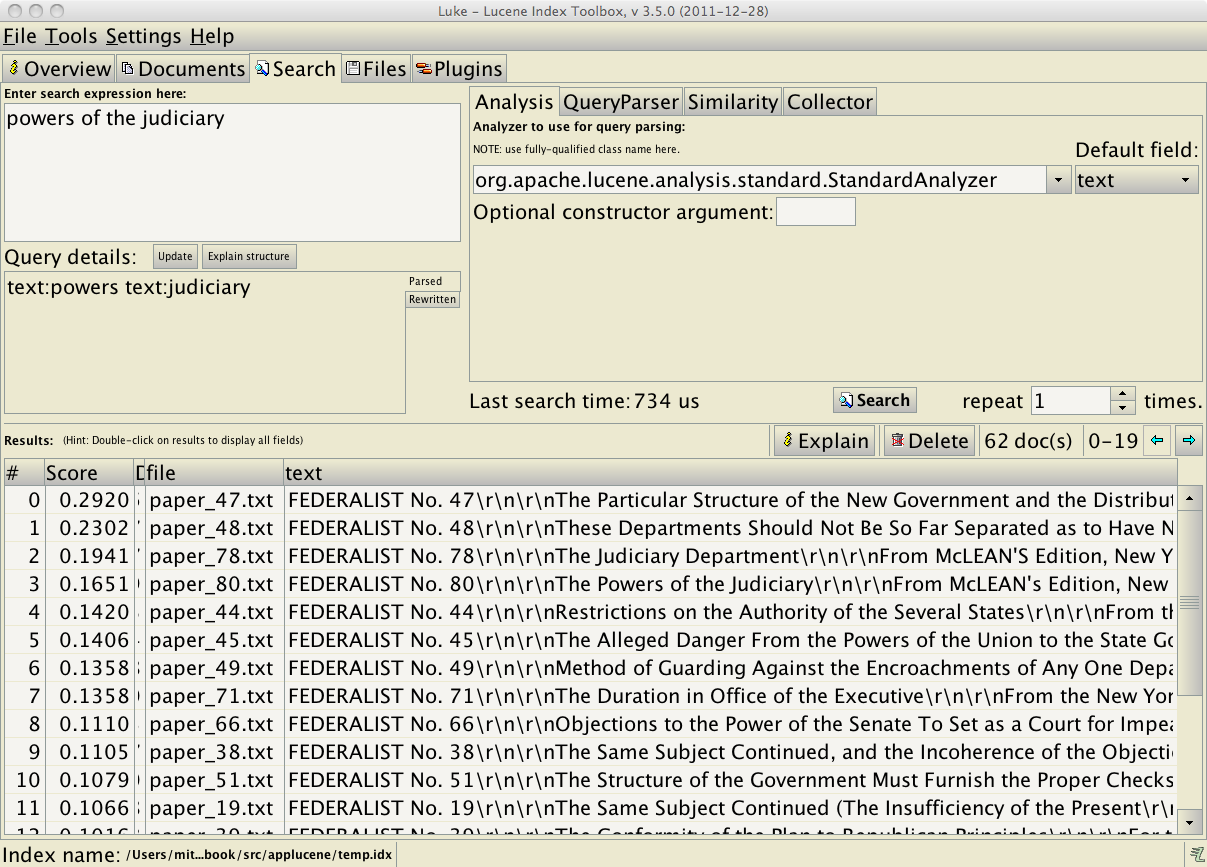
\includegraphics[width=5.1in]{pngs/luke2.png}
%\end{center}%
\vspace*{-18pt}
\caption{Screenshot of Luke index brower, showing search results}\label{fig:luke-search}
\end{figure}

\section{Search}

\subsection{Index Readers}

Lucene uses instances of the aptly named \code{IndexReader} to
read data from an index.

\subsubsection{Distributed Readers}

A convenient feature of the reader design in Lucene is that we may
construct an index reader from multiple indexes, which will then
combine their contents at search time.  From the reader's client's
perspective, the behavior is indistinguishable (other than in terms of
speed) from a combined and optimized index.  We can even distribute
these indexes over multiple machines on a network using Java's Remote
Method Invocation (RMI).


\subsection{Index Searchers}

Lucene supplies an \code{IndexSearcher} class that performs the actual
search.  Every index searcher wraps an index reader to get a handle
on the indexed data.  Once we have an index searcher, we can supply
queries to it and enumerate results in order of their score.

There is really nothing to configure in an index searcher other
than its reader, so we'll jump straight to the demo code.

\subsection{Search Demo}\label{section:lucene-search}

We provide a simple implementation of Lucene search based on the index
we created in the last section.  

\subsubsection{Code Walkthrough}

The code is in the \code{main()} method of the demo class
\code{LuceneSearch}.  The method starts off by reading in command-line
arguments.
%
\codeblock{LuceneSearch.1}
%
We need the directory for the index, a string representing the query
in Lucene's query language, and a specification of the maximum number
of hits to return.  The method is declared to throw a Lucene corrupt
index exception if the index isn't well formed, a Lucene parse
exception if the query isn't well formed, and a general Java I/O
exception if there is a problem reading from or writing to the index
directory.

After setting the command-line arguments, the next step is to
create a Lucene directory, index reader, index searcher and
query parser.
%
\codeblock{LuceneSearch.2}
%
It is important to use the same analyzer in the query parser as is
used in the creation of the index.  If they don't match, queries that
should succeed will fail because the tokens won't match.%
%
\footnote{The analyzers must produce the same tokenization.
 In the demo programs here, the analyzer used to create the index
 was a \code{StandardAnalyzer} wrapped  in a 
 \code{LimitTokenCountAnalyzer}.
 Since the \code{LimitTokenCountAnalyzer} doesn't change the underlying
 tokenization and we don't expect our queries to be very long,
 the query parser uses a \code{StandardAnalyzer}.}
%
For instance, if we apply stemming in the indexing to reduce
\stringmention{codes} to \stringmention{code}, then we better do the
same thing for the query, because we won't find \stringmention{codes}
in the index, only its stemmed form \stringmention{code}.

The last bit of code in the search demo uses the query parser to parse
the query, then searches the index and reports the results.
%
\codeblock{LuceneSearch.3}
%
The \code{Query} object is created by using the parser to parse the
text query.  We then use the searcher instance to search given the
query and an upper bound on the number of hits to return.  This
returns an instance of the Lucene class \code{TopDocs}, from package
\code{search}, which encapsulates the results of a search (through
references back into the index).

The \code{TopDocs} result provides access to an array of search
results.  Each result is an instance of the Lucene class
\code{ScoreDoc}, also in the \code{search} package, which
encapsulates a document reference with a floating point score.

The array of search results is sorted in decreasing order of score,
with higher scores representing better matches.  We then enumerate
over the array, and for each \code{ScoreDoc} object, we pull its score
out using the public member variable \code{score}.  We then pull its
document reference number (Lucene's internal identifier for the doc)
out with the member variable \code{doc}.  With the Lucene document
identifer, we are able to retrieve the document from the searcher
(which just delegates this operation to its index reader internally).
Finally, with the document in hand, we retrieve its file name using
the \code{get()} method on the document; we use \code{get()} here
rather than \code{getValues()}, which returns an array, because we
know there is only one file name for each document in the index.  We
could've also retrieved the text of the document, because we stored it
in the index.

\subsubsection{Running the Demo}

The Ant target \code{lucene-search} invokes the demo with command-line
arguments provided by the value of properties \code{index.dir},
\code{query}, and \code{max.hits}.
%
\commandlinefollow{ant -Dindex.dir=temp.idx -Dquery="powers of 
the judiciary" -Dmax.hits=15 lucene-search}
\begin{verbatim}
Index Dir=/Users/mitzimorris/aliasi/lpbook/src/applucene/temp.idx
query=powers of the judiciary
max hits=15
Hits (rank,score,file name)
  0 0.29  paper_47.txt
  1 0.23  paper_48.txt
  2 0.19  paper_78.txt
...
 13 0.10  paper_81.txt
 14 0.09  paper_82.txt
\end{verbatim}
%
We run this demo with the query string \stringmention{powers of the judiciary}.
As we saw in the previous section, the query parser stop-lists
the words \stringmention{of} and \stringmention{the}, reducing this
query to a boolean search for documents which contain the terms
\searchquery{text:powers} and/or \searchquery{text:judiciary}.
Lucene returns 15 results numbered 0 to 14.  We see that paper 47 is
the closest match to our query.  This
document contains 18 instances of the term \stringmention{powers} and
24 instances of \stringmention{judiciary}.  This seems like a low score on a 0--1 scale
for a document which matches all the tokens in the query; the reason
is because the documents are long, so the percentage of tokens in
the doucment matching the query tokens is relatively low.

The token \stringmention{food} does not show up in any documents, so
the query \searchquery{text:food} returns no hits.  If we enter the query string
\stringmention{powers of the judiciary food}, it returns exactly the same hits as
the query string \stringmention{powers of the judiciary}, in exactly the same order, but with
lower scores.  If we try the query string \stringmention{judiciary +food}, we are
insisting that the token \stringmention{food} appear in any matching
document.  Because it doesn't appear in the corpus at all, the query string
\stringmention{judiciary +food} has zero hits.  On the other hand, the
must-not query \stringmention{judiciary -food} has the same hits with the
same scores as does the query for \stringmention{judiciary}.


\subsection{Ranking}

For scoring documents against queries, Lucene uses the complex and
highly configurable abstract base class \code{Similarity} in the
package in \code{org.apache.lucene.search}.  If nothing else is
specified, as in our simple demos, the concrete subclass
\code{DefaultSimilarity} will be used.

Similarity deals with scoring queries with \code{SHOULD}-occur terms.
In the search language, all tokens are treated as \code{SHOULD}
unless prefixed with the must-occur marking plus-sign
(\code{+}) or must-not occur negation (\code{-}).

The basic idea is that the more instances of query terms in a document
the better.  Terms are not weighted equally.  A term is weighted based
on its inverse document frequency (IDF), so that terms that occur in
fewer documents receive higher weights.  Weights may also be boosted
or lowered in the query syntax or programatically with a query object.

All else being equal, shorter documents are preferred.
The reason for this is that when two documents contain the same number of
instances of query terms, the shorter document has a higher proportion of query
terms and is thus likely to be a better match.
This proportion may well be higher for a short document which contains only
a few instances of the query term than it is for a very long document which
contains many instances of the query term.
This can be problematic when a document collection contains both
very short and very long documents.

There is also a component of scoring based on the percentage of the
query terms that appear in the document.  All else being equal, we
prefer documents that cover more terms in the query.


\section{Deleting and Updating Documents}\label{section:lucene-delete}

The the \code{IndexWriter} class supports methods to delete documents
from an index based on a term or query.
There is also a \code{deleteAll()} method to completely clear the index.

In early versions of Lucene, document deletion was handled by
an \code{IndexReader}.%
%
\footnote{Because the \code{IndexWriter} was originally designed just
  to append documents to an existing index, it didn't need to keep
  track of documents already in the index.  But in order to delete a
  document, first it must be found.  Since this couldn't be done
  with an \code{IndexWriter}, the \code{deleteDocument} methods were
  added to the \code{IndexReader} class.}
%
However, as of 3.6 these delete document(s) methods on \code{IndexReader} have
been deprecated and in Lucene 4.0 all write support for this class will be removed.

The the \code{IndexWriter} class supports methods to update a document
or documents that contain a term.  The update operation consists of first
deleting the existing document(s) which contain a given term and then
adding new one(s).  This operation is atomic with respect to any index
readers open on the index.

In many cases, the documents being indexes have unique identifiers.
For example, in our file-based index, the file names are meant to be unique.%
%
\footnote{Unlike a database, which enforces unique ids by declaration,
Lucene requires the programmer to treat fields as keys by convention.}
%
We can then create a term containing the application's document
identifier field and delete by term.  For instance, we could call
\code{deleteDocuments(new Term("file","paper\_12.txt"))} to delete the
document with file identifier \code{paper\_12.txt}.

\subsection{Visibility of Deletes}

When a delete method is called on a writer based on a term
or document identifier, the documents are not immediately physically
deleted from the index.  Instead, their identifiers are buffered and
they are treated as if virtually deleted.  

This approach to document deletion was made for the same efficiency
reasons and faces many of the same issues as concurrent sets of
variables in Java's memory model.  Even when deletes are called on one
index, not every reader with a handle on that index will be
able to see the delete, but any new reader opened on the index after the
delete will see the deletion.

The storage space for a deleted document in the index directory is
only reclaimed during a merge step.

\subsection{Lucene Deletion Demo}

We have implemented an example of deleting documents in the 
demo class \code{LuceneDelete}.

\subsubsection{Code Walkthrough}

The code is entirely straightforward, with the \code{main()} method
taking three command-line arguments, the index directory path, along
with the field name and token used to construct the term to delete.
We open the index directory and create a default analyzer just as
we did in the demo class \code{LuceneIndexing}.
%
\codeblock{LuceneDelete.1}
%
We create an \code{IndexWriterConfig} object that will be passed
in to the \code{IndexWriter} constructor, but this time
we set the open mode to
\code{IndexWriterConfig.OpenMode.APPEND}.
%
\codeblock{LuceneDelete.2}
%
We then construct a term out of the field and token and pass it to
the index writer's delete method.  After the deletion, we query the
writer to find out if deletions are pending.
We check the number of docs before and after the call to the \code{commit()} method.

\subsubsection{Running the Demo}

The Ant target \code{lucene-delete} invokes the class, supplying
the value of properties \code{index.dir}, \code{field.name}, and
\code{token} as command-line arguments.  

Make sure that before you run this demo, you've run the indexing
demo exactly once.  You can always delete the index directory and
rebuild it if it gets messed up.
%
\commandlinefollow{ant -Dindex.dir=temp.idx -Dfield.name=file -Dtoken=paper\_12.txt lucene-delete}
\begin{verbatim}
index.dir=/Users/mitzimorris/aliasi/lpbook/src/applucene/temp.idx
field.name=file
token=paper_12.txt
Num docs before delete=84
Has deleted docs=true
Num docs after delete before commit=84
Num docs after delete=84
\end{verbatim}

After the demo is run, we can look at the index directory again.
%
\commandlinefollow{export BLOCKSIZE=1024; ls -1 -s temp.idx}
\begin{verbatim}
total 1524
1144 _0.fdt
   4 _0.fdx
   4 _0.fnm
  84 _0.frq
   4 _0.nrm
 188 _0.prx
   4 _0.tii
  80 _0.tis
   4 _0_1.del
   4 segments.gen
   4 segments_2
\end{verbatim}
%
There is now an extra file with suffix \code{.del} that holds
information about which items have been deleted.  These deletes will
now be visible to index readers that open (or re-open) their
indices.  The file containing the deletions will be removed, and the
actual content deleted, when the index is merged or optimized by an
index writer.


\section{Lucene and Databases}

Lucene is like a database in its storage and indexing of data in a
disk-like abstraction.  The main difference between Lucene and a
database is in the type of objects they store.  Databases store
multiple type-able tables consisting of small data objects in the
rows.  The Structured Query Language (SQL) is then used to retrieve
results from a database, often calling on multiple tables to perform
complex joins and filters.  

Lucene, on the other hand, provides a configurable, but more
homogeneous interface.  It mainly operates through text search (with
some lightweight numerical and date-based embellishments), and
returns entire documents.%
%
\footnote{Nothing prevents us from treating paragraphs or even sentences in a
``real'' document as a document for Lucene's purposes.}

\subsection{Transactional Support}

In enterprise settings, we are usually very concerned with maintaining
the integrity of our data.  In addition to backups, we want to ensure
that our indexes don't get corrupted as they are being processed.

A transaction in the database sense, as encapsulated in the Java 2
Enterprise Edition (J2EE), is a way of grouping a sequence of complex
operations, such as committing changes to an index, such that they all
happen or none of them happen.  That is, it's about making complex
operations behave as if they were atomic in the concurrency sense.

Earlier versions of Lucene were not like databases in not having any
kind of transactional support.  More recently, Lucene introduced
configurable commit operations for indexes.  These commit operations
are transactional in the sense that if they fail, they roll back any
changes they were in the middle of.  This allows standard
database-type two-phase commits to be implemented directly with
fine-grained control over preparing and rolling back.

 







